\section{Results}
The simulations follow a similar pattern to what \cite{de2010multi} did.
First a social network of new agents is created and than the simulation is started.
In every iteration a random agent is select from the network and shifts a random trajectory.
It then plays 100 \textit{Imitation Games} with every friend it has, to get a success value of this shifted trajectory.
After these games, an accept or reject is done based on the number of successful \textit{Imitation Games}.
If the trajectory is accepted, a mix between the original trajectory and the shifted trajectory is made and stored in the agent (the success value for this trajectory is also updated as seen in \citep{de2010multi}).
After this is done, the agent has a \textit{falling out} with one of its friends (if it has more then two) based on the success of the \textit{Imitation Game} the two agents played.
Finally, the agent is presented with a new friend via the FoaF method where a friend of the agent, suggest a new friend.
And then the next iteration starts.

\begin{table}[t]
    \centering
    \begin{tabular}{ll}
    \hline
    Parameter                                         & Value  \\ \hline
    Number of Iterations ($N_{iterations}$)           & 600000 \\
    Number of games ($N_{test}$)                      & 100    \\
    $\sigma_{noise}$                                  & 2.0    \\
    $\sigma_{shift}$                                  & 1.0    \\
    mix-factor ($\beta$)                              & 0.5    \\
    Number of agents                                  & 100    \\
    Number of trajectories                            & 4      \\
    Trajectory length                                 & 20     \\
    Maximum distance between neighboring points ($R$) & 1.0    \\
    Space size                                        & 10     \\
    Average number of friends                         & 10    
\end{tabular}
    \caption{Table to test captions and labels.}
    \label{table:simulation}
\end{table}

\begin{figure}[t]
    \centering
    \begin{subfigure}[t]{0.35\textwidth}
        \centering
        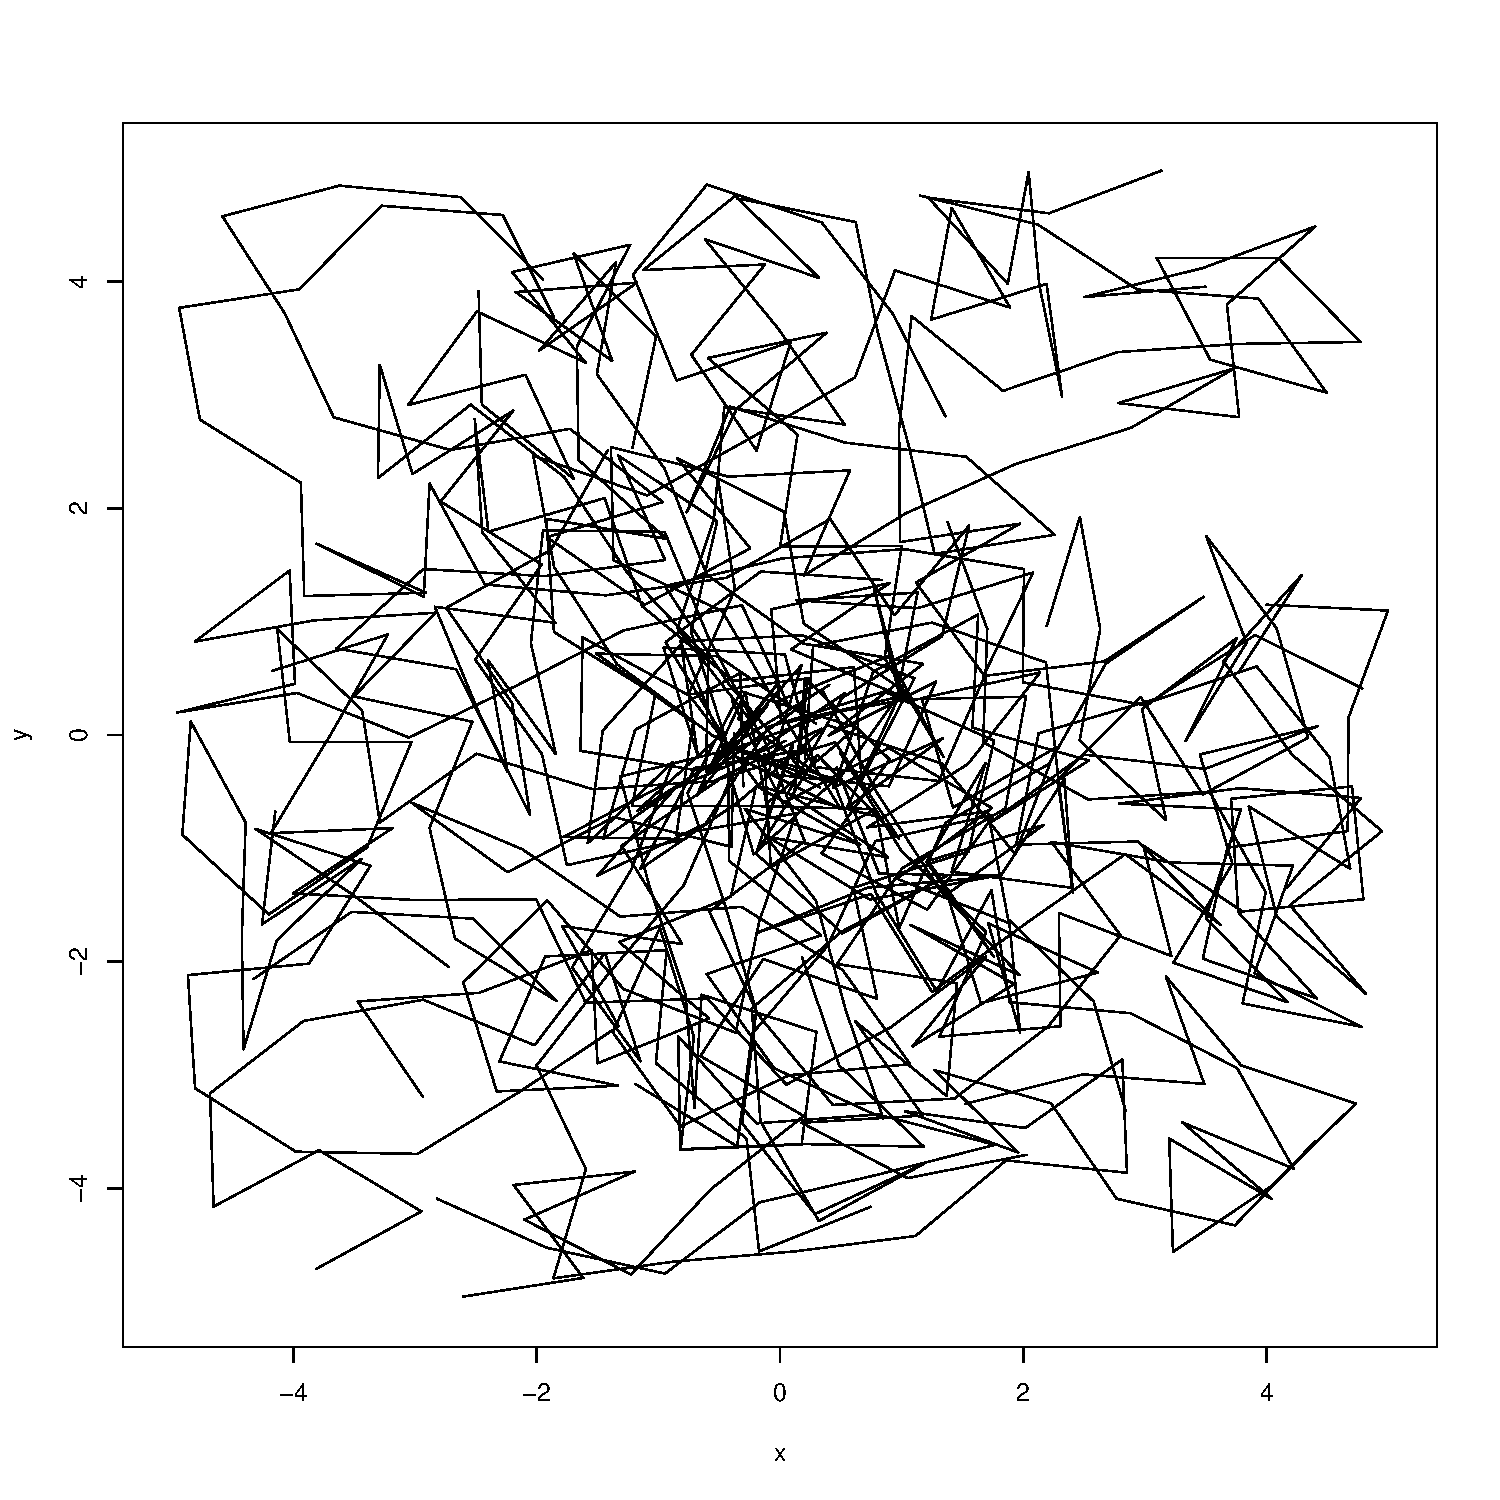
\includegraphics[width=\textwidth]{friendInit.pdf}
        \caption{Initial trajectories of ten random agents from the social network before the simulation starts.}
        \label{fig:FriendInit}
    \end{subfigure}
    \hfill
    \begin{subfigure}[t]{0.35\textwidth}
        \centering
        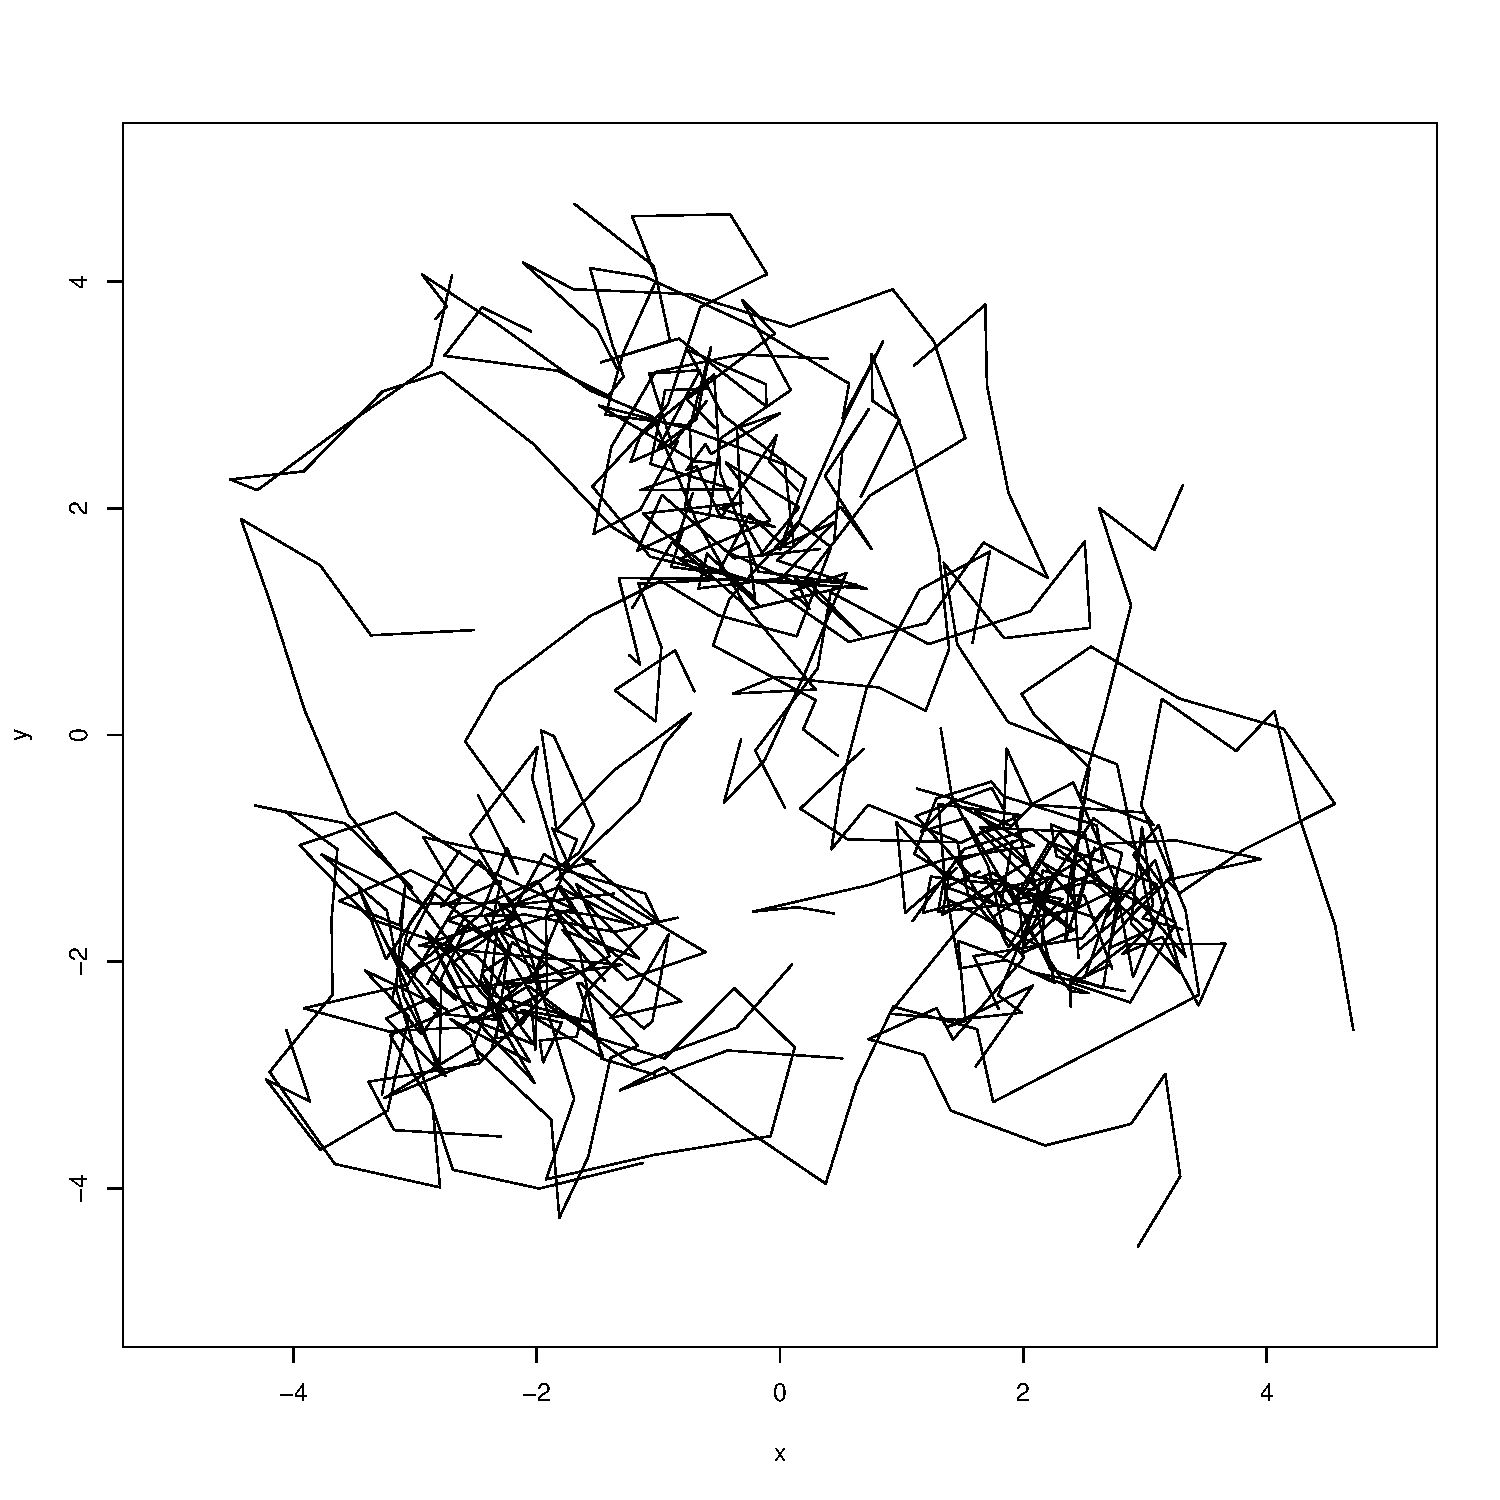
\includegraphics[width=\textwidth]{friendOut.pdf}
        \caption{The resulting trajectories of the ten randomly selected agents after the simulation.}
        \label{fig:friendRes}
    \end{subfigure}
    \hfill
    \begin{subfigure}[t]{0.5\textwidth}
        \centering
        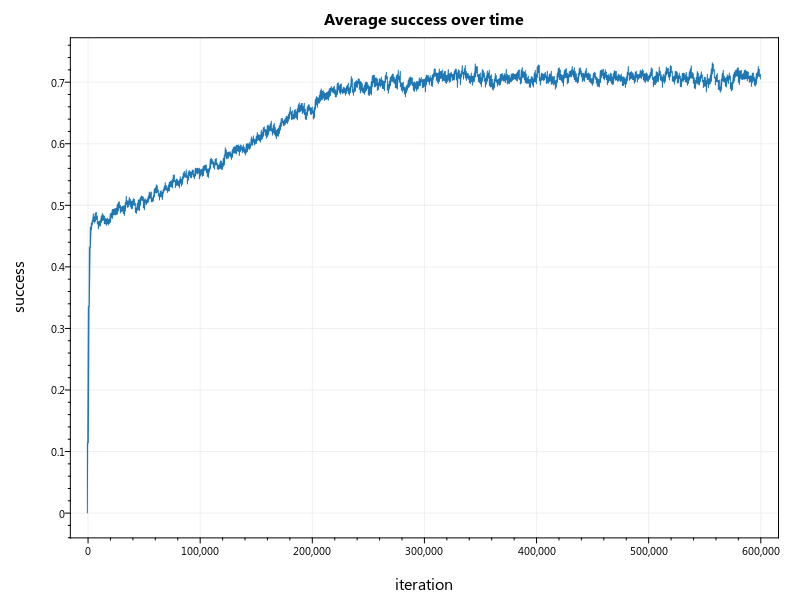
\includegraphics[width=\textwidth]{friendSuccess.png}
        \caption{The running average success of the simulation.}
        \label{fig:friendSuccess}
    \end{subfigure}

    \caption{Both (a) and (b) show the trajectories of ten randomly selected agents before and after 600.000 iterations.}
    \label{fig:friend}
\end{figure}
The results presented in the paper where achieved by running the simulation with the values found in \autoref{table:simulation}.
Most of the values are identical to the simulation parameters found in \citep*{de2010multi}.
The results are summarised in \autoref{fig:friend}.
\autoref{fig:FriendInit} and \autoref{fig:friendRes} are trajectories of 10 random agents before and after te simulation, and serve as a small small in which we analyze the results.
Plotting 100 agents would be even more chaos and because of the random sample, it should represent the stated of the population a bit.

\begin{figure}[t]
    \centering
    \begin{subfigure}[t]{0.35\textwidth}
        \centering
        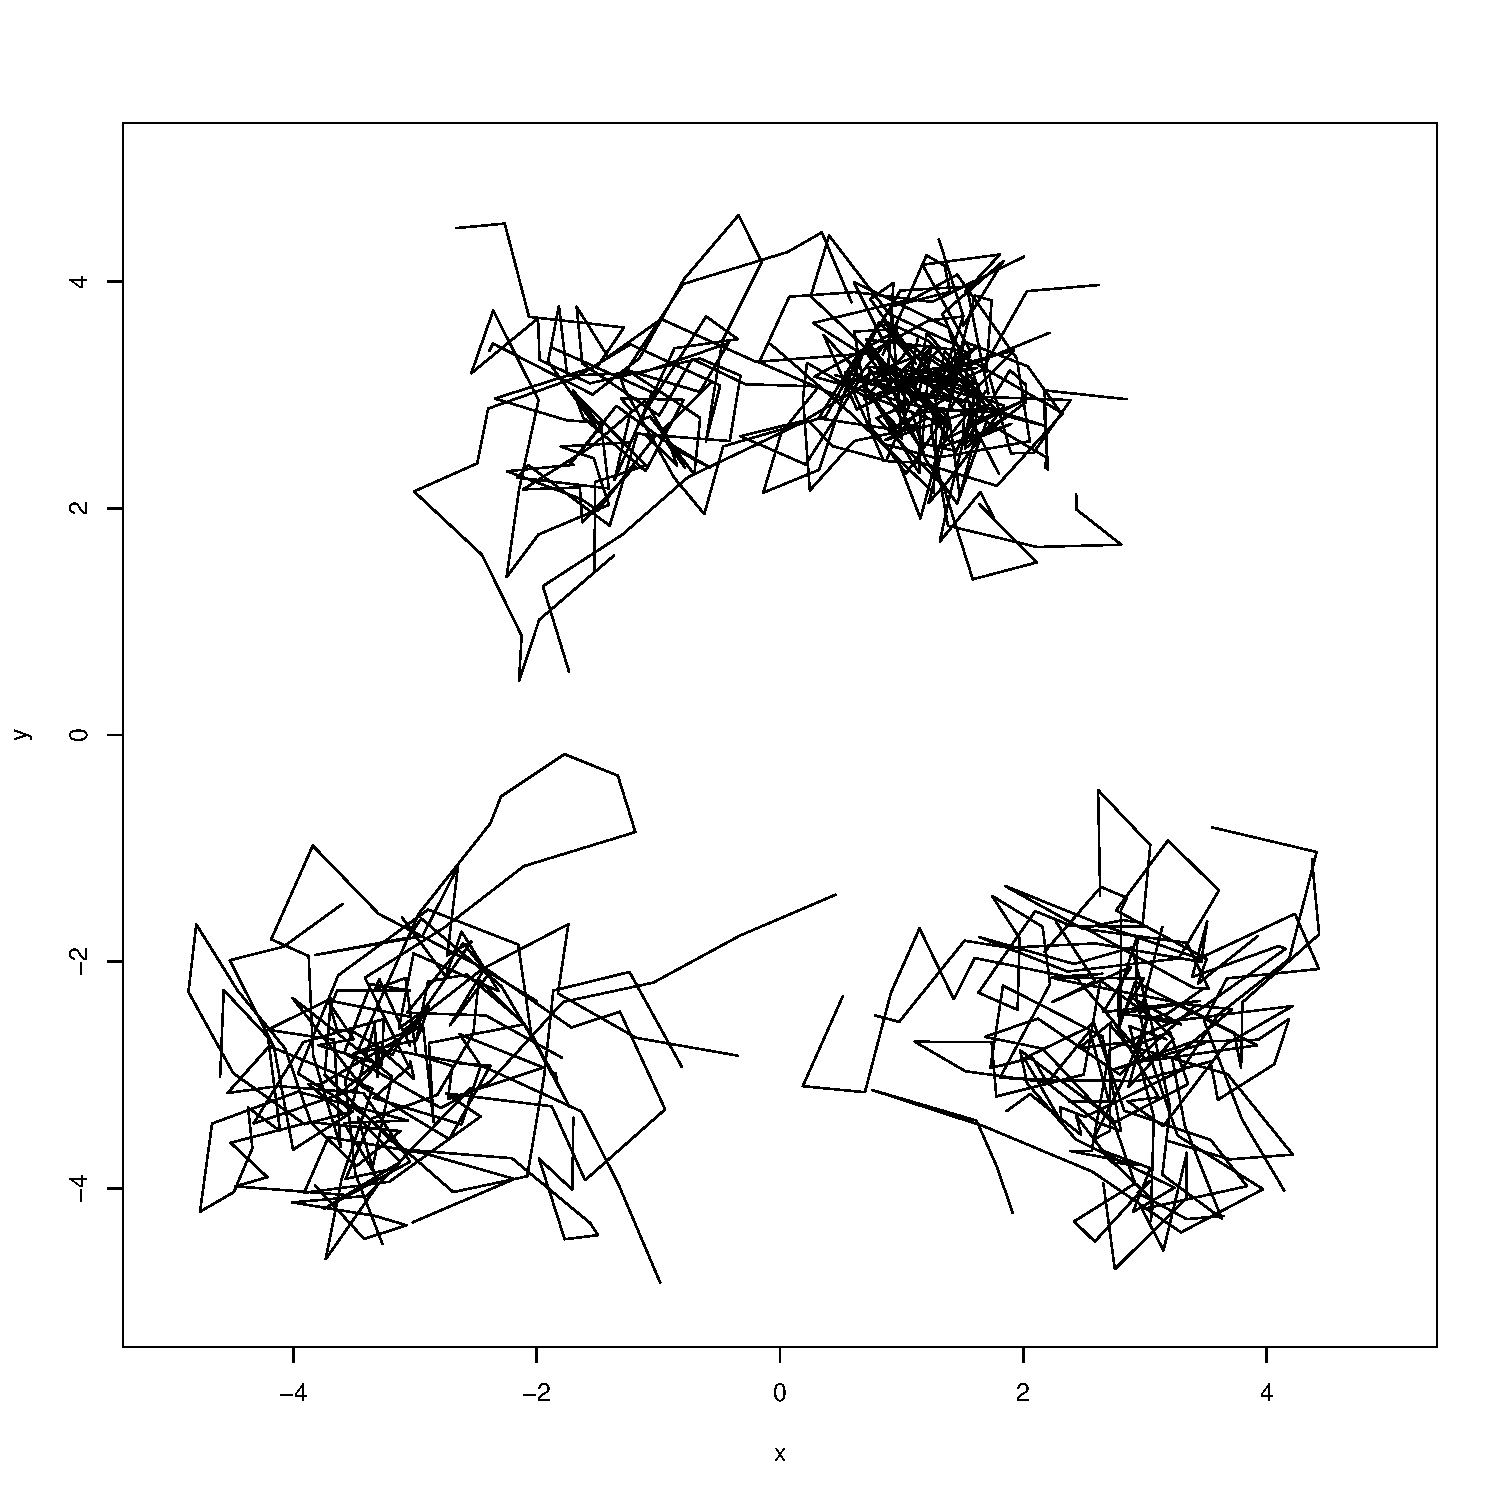
\includegraphics[width=\textwidth]{out_T4_100.pdf}
        \caption{The resulting trajectories of 10 random agents.}
        \label{fig:Traject4Res100}
    \end{subfigure}
    \hfill
    \begin{subfigure}[t]{0.45\textwidth}
        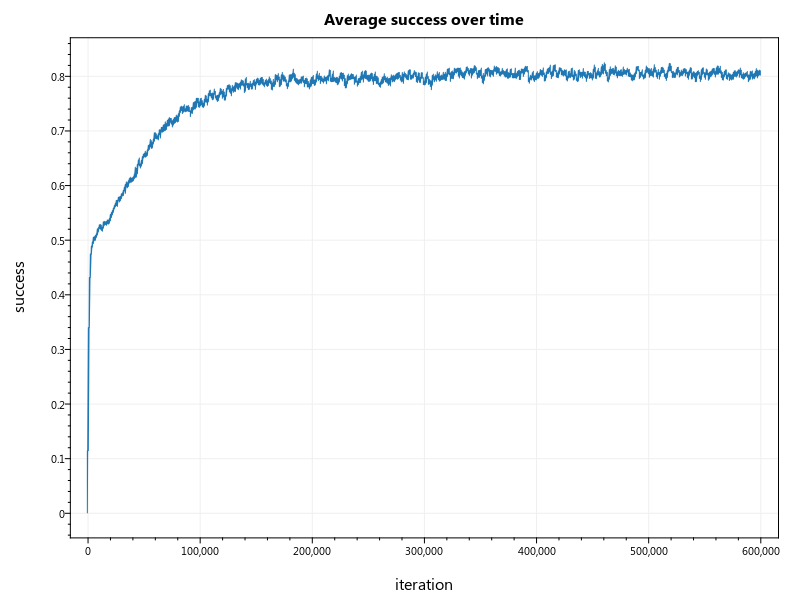
\includegraphics[width=\textwidth]{success_T4_100.png}
        \caption{The running average success of the simulation}
        \label{fig:Traject4Success100}
    \end{subfigure}

    \caption{Some the results of running the original model but with 100 agents instead of 10 (for 600.000 iterations).}
    \label{fig:Traject4_100}
\end{figure}

Looking at the results in more detail, the first thing to note is \autoref{fig:friendSuccess}.
Here a similar trend is observed as seen in \autoref{fig:Traject4Success}, with the major difference being that the trend takes 10 times more iterations before it starts to stagnate compared to the method of \cite{de2010multi}.
It might seem obvious because of the method presented tests with 100 agents but this is not entirely true.
Running the original project with 100 agents and for 600.000 iteration, a similar trend can be seen as presented in \autoref{fig:Traject4Success100}.
10 times more agents also means more then 10 times longer for the population to settle.

\autoref{fig:Traject4Res100} shows that around 200.000 iteration the success rate starts to stagnate, where as the model presented here starts to stagnate at around 300.000.
This is due to the fact that changing social network prevent a faster spread of shifted trajectories.
A shift that is tested against every agent in the population is more certain that it can be accepted or rejected, whereas a shifted trajectory that is only tested against a few agents in the population local optima creates.
Acceptance is thus dictated by the connections an agent posses.


Inspecting the results a bit more, it becomes clear that distinctness is harder to come by and this is shown in \autoref{fig:friendRes}.
There should be four trajectories, but only three clusters show up and are relative close to each other, compared to \autoref{fig:Traject4Res}.
The main reason is clearly the changing social network but the number of agents in the population plays some roll as seen in \autoref{fig:Traject4Res100} where the four clusters are clearly visible but the two on top are very close to each other.


